\documentclass[letterpaper,titlepage,12pt]{article}

\usepackage{setspace}
	\doublespacing
    \frenchspacing
\usepackage[margin=0.9in]{geometry}
\usepackage{fancyhdr}

    \pagestyle{fancy}
    \setlength{\headheight}{15pt}
    \rhead[Emily Che]{Emily Che}
    \lhead[]{}



\usepackage{textcomp}


\setcounter{secnumdepth}{3}

\widowpenalty=300
\clubpenalty=300
%\title{Thesis Proposal}
\title{Thesis proposal: Population diversity of  \textit{Campylobacter jejuni} in a southern Ontario raccoon population}
\author{Emily Che}
\date{June 2020}

\usepackage[
    backend=biber,
    style=authoryear,
    sorting=nyt
]{biblatex}

\addbibresource{References.bib}
\usepackage{lineno}
\usepackage{siunitx}
\usepackage{graphicx}


\begin{document}

\maketitle
\linenumbers
\section{Summary}



\textit{Campylobacter} is the leading cause of bacterial gastroenteritis worldwide. Typically, investigations of Campylobacter have focused on poultry or other farm animals due to their importance in transmission to humans. There is a lack of research into other species, particularly wildlife species, that are capable of harbouring \textit{Campylobacter}. Raccoons (\textit{Procyon lotor}) are commonly found throughout North America and are found in rural and urban environments. Additionally, raccoons are capable of moving between these different environments. Raccoons have been found to harbour \textit{Campylobacter jejuni}, including raccoon-specific strains and generalist strains that have been found in other sources, including clinical cases. 

In Canada, surveillance of \textit{Campylobacter} is limited.  There has been little research into how \textit{Campylobacter} behaves in a population and the epidemiology of \textit{Campylobacter} remains unclear. Understanding the genomic diversity and carriage of strains of \textit{Campylobacter} within a southern Ontario raccoon population previously under study may provide a better understanding of \textit{Campylobacter} dynamics within a population. I hypothesize the approaches developed to analyze the \textit{Campylobacter}-positive raccoon population will be applicable to the analysis of population-level DNA genome sequence data from other sources of \textit{Campylobacter}, including humans. 

%what we are trying to do
% understand how campylobacter behaves within a pop -> genomic diversity, survival time, carriage, potential for colonization



The objectives of this research proposal are to develop analytical approaches to:

1. Investigate the population structure of \textit{Campylobacter jejuni} in a raccoon population.

2. Investigate the strain dynamics of \textit{Campylobacter jejuni} in the southern Ontario raccoon population.

\newpage
\section{Background} %fine

%Campy background
%   - symptoms and illness, relevance to humans, how humans get it 

%% Raccoons and 
% communal latrines, habitat, movment, pathogen relevance, previous studies that hae found campy in raccoons and their significance
%take out communal latrines? 


%carriage of campy
% genomic diversity of campy 

%WGS of raccoons as a tool? talk about surveillance of campylobacter esp in humans, use it as a method for developing approaches to WGS in humans, so talk about the usage of WGS

%risk of wildlife to agricultural plants too

% fine from here to the next comment
\textit{Campylobacter} is a ubiquitous foodborne bacterial pathogen, with the most important species to human health being \textit{Campylobacter jejuni}, followed by \textit{Campylobacter coli}  \parencite{mutschall2020campylobacter}. Campylobacteriosis, a gastroenteritis disease is estimated to cause 400-500 million cases worldwide per year \parencite{DuongTri2009CsoC}. 
In Canada alone, there are an estimated 447.23 campylobacteriosis cases per \SI{100000} people each year \parencite{thomas2013estimates}. While the majority of campylobacteriosis cases are mild, severe cases may lead to complications such as Guillain-Barr\'e Syndrome or death \parencite{DuongTri2009CsoC}. However, as most cases are self-limiting, most infections go undiagnosed or under-reported and outbreaks are considered sporadic \parencite{MaganaMaria2017Iitg, ravel2016non}. 

\textit{Campylobacter} is capable of colonizing a wide array of animals, including farm animals, domestic animals, and wild birds, and is also be found in the environment in water and soil \parencite{oh2018frequent}. Transmission of \textit{Campylobacter} is through the fecal--oral route \parencite{kaakoush2015global}. 
The main routes of transmission of \textit{Campylobacter} to humans are through the ingestion of contaminated food and water \parencite{kaakoush2015global}. Typically, humans become sick with \textit{Campylobacter} after ingesting contaminated and improperly prepared poultry products \parencite{newell2017campylobacter}.
%maybe revise the bottom?
Due to the importance of farm animals in transmission of \textit{Campylobacter} to human health, there has been limited research into the role of wildlife in transmission of \textit{Campylobacter}. However, wild animals have been implicated in spreading foodborne pathogens between farm animals and agricultural crops \parencite{erickson2016overview}. To date, the role of wildlife in \textit{Campylobacter} epidemiology remains unclear. However wild animals, such as raccoons, are increasingly being identified as potential reservoirs important to human infection \parencite{mutschall2020campylobacter, BondoKristinJ2019SCCd, lee2011summary, viswanathan2017molecular}. 



 Raccoons are capable of harbouring a number of enteric pathogens relevant to humans, including \textit{Campylobacter, Salmonella}, and \textit{Escherichia coli} \parencite{bondo2016impact, jardine2012antimicrobial, bondo2016epidemiology}. \textit{Salmonella} serovars found in feces of raccoons have also been implicated in infecting humans and livestock \parencite{bondo2016impact}. These findings indicate that raccoons living near humans and livestock may play a role in the transmission of \textit{Salmonella}. Raccoons may play a similar role in the transmission of \textit{Campylobacter}. In a previous study conducted on a population of raccoons in southern Ontario, raccoons were found to harbour \textit{C. jejuni} that were raccoon-exclusive strains and generalist strains \parencite{mutschall2020campylobacter}. The generalist \textit{C. jejuni} strains found in the raccoons have been found in other sources, including both agriculture and clinical cases. 

Raccoons in North America are well-adapted to urban and rural environments. Raccoons use human buildings for shelter and obtain resources from urban lawns and gardens, and have access to farmlands \parencite{rosatte2010density}. Raccoons are opportunists and will scavenge for food from human garbage. In rural settings, raccoons feed on chickens, farm feed, and agricultural crops \parencite{tyler2015notes}. Food opportunities may provide a way for raccoons to acquire \textit{Campylobacter}. Through shedding \textit{Campylobacter} in their feces, raccoons may contaminate the environment and food sources \parencite{BondoKristinJ2019SCCd}. On average, raccoons in Ontario range about \SIrange[range-units=single]{1}{4}{\km} on average, although raccoons in rural habitats range further than their urban counterparts \parencite{rosatte2000management, rosatte2010density}. Movement between different settings and between farms may provide a way for raccoons to facilitate the spread of \textit{Campylobacter}.   %Raccoons have behaviours that possibly aid in spreading pathogens and parasites amongst raccoon populations. Communal latrines with repeated defecation are used by raccoons \parencite{hirsch2014patterns}, and will "wash" their food in water before eating \parencite{SommerVolker2016Nela}.  

 %Raccoons may be colonized with species-adapted \textit{C. jejuni} \parencite{viswanathan2017cluster}. 
% definitely need to condense this raccoon secton 
   %In a study on raccoons in southern Ontario, the prevalence rate of 628 captured raccoons was 40.8\% \parencite{mutschall2020campylobacter}.
   
   
Although rare, raccoons have been identified as a source of infection for humans. In 2013, a human outbreak of campylobacteriosis at a Minnesotan wildlife centre was traced to the raccoons housed there \parencite{saunders2017outbreak}. However, several workers were not in contact with raccoons, suggesting environmental contamination by raccoons also played a role in transmission \parencite{saunders2017outbreak}. 

In the 2013 Minnesotan wildlife centre outbreak, identifying the source of outbreak was not complicated due to the unusual source and patients' history. However, because campylobacteriosis cases are usually widespread and sporadic, and \textit{Campylobacter} is so commonly found in many animals and in the environment, identifying the source of infection remains difficult \parencite{carrillo2012}. Further, the usual methods of subtyping are unable to provide enough discriminatory power to differentiate closely related isolates and identify if a strain is responsible for an outbreak.  

Whole genome sequencing has been applied to the surveillance of foodborne illnesses and outbreak investigation in foodborne pathogens. Whole genome sequencing technology is rapidly replacing other typing tools due to its ability to differentiate between close phylogenetic neighbours \parencite{MaganaMaria2017Iitg}. Whole genome sequencing provides higher discriminatory power than typical subtyping methods, such as multi locus sequence typing or comparative genomic fingerprinting. While the subtyping methods are able to cluster related strains, these methods fail to distinguish as to whether related samples are indeed the same strain. 

As the use of whole genome sequencing becomes more common, developing general approaches to analyzing \textit{Campylobacter} sequence data is important. In order to apply whole genome sequencing to detect and interpret genetic variation amongst strains, an understanding of the genomic diversity of \textit{Campylobacter} within a population is necessary. To determine if isolates share a source or are clonal isolates, understanding the baseline genomic diversity for a population is important \parencite{llarena2017whole, MaganaMaria2017Iitg}. Use of whole genome sequence data in outbreak detection depends on understanding the degree of variation within a population to determine if isolates represent the same strain. However, having enough data on a \textit{Campylobacter} population to understand a baseline genomic diversity can prove to be a challenge, particularly from sources such as humans. Surveillance of \textit{Campylobacter} in humans is limited, as samples are only collected when human outbreaks occur and, even then, only when experiencing symptoms serious enough to seek medical help \parencite{janiec2012laboratory, joensen2020whole}. Previous population level studies of \textit{Campylobacter} have been conducted using conventional subtyping data \parencite{Kwan5130, gruntar2015campylobacter}. 

\textit{Campylobacter} sequencing has primarily centered on isolates sourced from human infections and farm animals. \textit{Campylobacter} sequencing studies often have limited isolates to sequence due to resource constraints, and are unable to investigate population dynamics of \textit{Campylobacter} \parencite{cantero2018characterization, whitehouse2018use, clark2016genomic, kovanen2014multilocus}. Longitudinal population studies of \textit{C. jejuni} using whole genome sequencing are rare. 

%Additional advantages to using whole genome sequencing includes condensing various methodologies into a single workflow, such as species identification, subtyping, and antimicrobial testing \parencite{ribot2019}. Adoption of whole genome sequencing has been introduced by Pulsenet as a gold-standard method for use in surveillance of foodborne illnesses \parencite{ribot2019}.

% use for discriminatory power between unrelated strains and related strains 
%recombination affects the population structure of campy the most (compared to mutation). some strains appear to be clonal and will be linked by typing methods despite true differences in gene content between isolates and absence of epi links (from carrillo paper)

 % maybe include this more in the beginning to have it as an oh look we're using this 
% MaganMaria: The CGF is the preferred method for the detection of Campylobacter genes with high variability among the different species of bacterial clusters that have been previously identified by the MCGH method

%Whole genome sequencing has been applied to \textit{Listeria monocytogenes} cases. \textit{Listeria} which, similarily to \textit{Campylobacter}, causes sporadic cases and outbreaks through contaminated foods in humans.  Likewise, epidemiological data of \textit{L. monocytogenes} has been limited \parencite{lassen2016two}. 

%listeria were defined as the same outbreak strians if they belonged to the same sequence type with fewer than five SNP differences -> where did they arrive at 5 from? also seems like they were doing cgMLST -> chose it basd on situation-dependent evualtion of dendograms ----> may be how we have to do it with cmapy? 



% add more about surveillance on humans ---- need to tie it in more
% how many population level studies done on campy?
% level of genomic diversity already examined?



% other wildlife cases where animals have spread amongst farms and into produce
This thesis proposal aims to investigate \textit{Campylobacter} population dynamics in a raccoon population in order to further the understanding of how \textit{Campylobacter} behaves within a population, which I hypothesize may be applicable to other host populations.
%A raccoon population positive for \textit{C. jejuni} may help determine the degree of \textit{C. jejuni} genomic diversity within a population. 
Understanding the genomic diversity of \textit{Campylobacter} will help in understanding the epidemiology of the pathogen. In addition, understanding whether raccoons may be involved in \textit{Campylobacter} transmission may also further the understanding of the epidemiology of \textit{Campylobacter}. Specifically, using a raccoon population to investigate \textit{Campylobacter} dynamics will be useful for understanding \textit{Campylobacter} populations and developing approaches to analyzing sequence data of \textit{Campylobacter} to investigate campylobacteriosis in humans. 


% add hypotheses at the end:
% 1. population structure 
    % more genomic diversity in lineages that are more generalist vs raccoon exclusive
    % location -> farm more genomic diversity?
    % 
    % hypothesize that this dataset can be used as a model that will be applicable to human data (population data overall). 

\section{Objectives}

The objectives of this research proposal are to use the previously studied \textit{Campylobacter jejuni} positive raccoon population from southern Ontario as a model for analyzing strain dynamics in a population. I hypothesize the methods that will be developed will be applicable to analyzing sequence data of \textit{Campylobacter} from human campylobacteriosis cases. To investigate population dynamics in a \textit{Campylobacter} population, this proposal will address two main objectives: 

1. Investigate the population structure of \textit{Campylobacter jejuni} in a raccoon population through exploring the genomic diversity found within the population. 

2. Investigate the strain dynamics of \textit{Campylobacter jejuni} within the southern Ontario raccoon population. 



\section{Methods and Proposed Approach}

\subsection{Genome Sequence Collection}

\subsubsection{Animal sampling methods}  %fine
Sample collection and processing of \textit{Campylobacter} from raccoons occurred from May 2011 to November 2013. The trapping and handling of raccoons were approved by the Animal Care Committee at the University of Guelph and described in \cite{bondo2015longitudinal}. Fecal samples were collected by live-trapping raccoons on five swine farms and five conversation areas located in the Grand River Watershed in southern Ontario. Each site was trapped once every five weeks, using 20 to 40 Tomahawk live traps. Raccoons were anaesthetized to obtain fecal swabs and tagged to identify individuals. Individuals were sampled only once per monthly trapping week, however additional samples were taken from previously sampled individuals if caught in subsequent months. Location, date, weight, and age class was collected for each raccoon trapping. A total of 628 raccoons yielded 1096 trappings, of which 508 trappings were \textit{Campylobacter}-positive. 
%fine

\subsubsection{Isolation and \textit{Campylobacter} confirmation}

Isolation of \textit{Campylobacter} isolates was conducted over the course of three years, May 2011 to November 2013. Fecal swabs were sent to the Public Health Agency of Canada's laboratory at the Animal Diseases Research Insitute in Lethbridge, Alberta and individual colonies were isolated from fecal swabs. Isolation and culture of \textit{Campylobacter} samples was conducted as described in \cite{mutschall2020campylobacter}. In short, fecal swabs were submerged, mixed, and incubated in supplemented Bolton broth under microaerophilic conditions for 24 hours at 42\textdegree C. Broth cultures were then streaked onto modified blood-free charcoal cefoperazone deoxycholate agar and incubated for a futher 48 hours under the same conditions. 3-5 colonies per sample were subcultured onto blood agar and incubated. DNA was extracted from the colonies according to Qiagen's EZ1 DNA tissue kit. 
%fine

A multiplex polymerase chain reaction (PCR) was used to confirm \textit{Campylobacter} positive isolates and identify the species. The PCR targeted \textit{Campylobacter} genus-specific region of 16S rRNA gene, the \textit{mapA} gene for \textit{C. jejuni} and \textit{ceuA} for \textit{C. coli}  \parencite{denis1999development}. 502 out of 508 \textit{Campylobacter}-positive trappings were positive for \textit{C. jejuni}, the remaining 6 trappings were positive for \textit{C. coli}.



\subsubsection{\textit{Campylobacter} subtyping} %fine


Comparative Genomic Fingerprinting (CGF) is a multiplex PCR and was run on all confirmed \textit{Campylobacter} isolates. CGF subtyping is based on the presence and absence of 40 accessory genes using NCTC11168 as a control, and methods are described in \cite{Taboada788}. The presence of a gene is given a 1 and absence of a gene is given a 0. The combination of 1s and 0s provides a binary CGF subtype. A CGF subtype represents a genetic lineage, and is henceforth referred to as a CGF lineage. The Canadian Campylobacter Comparative Genomic Fingerprinting Database (C3GFdb) contains samples from across Canada and a variety of hosts, including farm, domestic, and wildlife animals, in addition to clinical cases and environmental samples. 1555 raccoon \textit{Campylobacter}-positive samples were subtyped and compared against the C3GFdb. 96 distinct CGF lineages were observed from the raccoon population, of which 46 were novel and therefore are considered raccoon-exclusive lineages. The remaining lineages were mainly generalists (mixed-hosts source attribution) with both agriculture and clinical associations, while a few lineages that were primarily clinically-associated \parencite{mutschall2020campylobacter}. 

\subsubsection{Whole Genome Sequencing}
% protocol -> public health agency

937 of \SI{1555} isolates were selected to be sequenced. To examine genomic diversity, isolates that were gathered from the same raccoon on the same trapping date were included for sequencing. To examine strain dynamics in the population, isolates that represented recapture events were also included. Isolates selected for sequencing represented different CGF lineages, which were raccoon-exclusive, generalist lineages, or clinically-associated lineages. Isolates that were selected were regrown as bacterial lawns on blood agar, and a loop of bacterial culture was taken for DNA extraction. DNA extraction was followed according to Public Health Agency of Canada's Whole Genome Sequencing protocol (DED-PR-015 DNA Extraction and Standardization, DED-PR-350 Genomics-Based Identification and Characterization of Enteric Bacterial Pathogens) using the Qiagen DNA extraction kit.
DNA was submitted to the Public Health Agency's Genomic Core for whole genome sequencing on Illumina's Nextseq platform. Sequence data was uploaded to the Integrated Rapid Infectious Disease Analysis platform (IRIDA) \parencite{Matthews381830}. IRIDA is a data management system for biological data that keeps track of data from sequencer to the results.

%Isolate selection was based on CGF lineages of interest (ie., lineages that were raccoon-exclusive, generalist lineages, clinically-relevant), and isolates that came from same raccoon-same date samplings and recapture events. 




\subsection{Genome assembly and preliminary analyses} %fine

Genomes will be assembled using \textit{de novo} assembly (SPAdes via Shovill pipeline). %Data cleaning and filtering of incomplete genomes will be conducted in R \parencite{R}. 
eCGF, which simulates CGF \textit{in silico}, will be used to subtype the genomes and used  to validate the isolates with wet-lab identity (https://www.github.com/dorbarker/CGFPrediction@improvements). Genomes where the eCGF subtype did not match with the previously ascertained CGF subtype will be discarded. Genomes with missing alleles will be attempted to be recovered using crowBAR \parencite{barker2018principles}. Core genome multi locus sequence typing (cgMLST) compares the genetic diversity of isolates by comparing the allelic diversity of loci found in all members of the species \textit{C. jejuni} \parencite{barker2018principles}. cgMLST will be used to% compare the genetic diversity of isolates by comparing  
conduct gene-by-gene comparisons in order to ascertain the similarity of genomes. Single Nucleotide Polymorphisms (SNP) will be used to highlight differences between highly-related genomes. SNP compares single base-pair differences in the genomes \parencite{petkau2017snvphyl}.
%add cgMLST and SNVphyl up here


\subsection{Population structure of \textit{C. jejuni} in a southern Ontario raccoon population}

The baseline genomic diversity of CGF lineages will be determined in order to consider whether related isolates represent the same strain using whole genome sequencing data. Determining the baseline genomic diversity is important for further analyses of the population. %The extent of co-infection within individual raccoons will be determined. -> move
After establishing the baseline genomic diversity, the overall population diversity will be examined. %A distance matrix will be generated based on genome-pair comparisons to examine genomic relatedness. 

\subsubsection{Establishing the similarity of isolates obtained from the same individual raccoon on the same collection date} %fine

779 genomes from 508 sampling events represent isolates that are from same raccoon and same sampling date events. Many isolates taken from the same raccoon on the same sampling date have the same CGF lineage, and therefore may be the same strain. First, similarity of isolates with the same lineage are from the same raccoon obtained at the same sampling time will be compared using a distance matrix. Similarity will then be compared between different raccoons under the same condition (same CGF lineage, genomes from same raccoon-same sampling date) in order to determine a threshold of similarity needed to be considered the same strain.  
Each CGF may lineage have its own degree of diversity, therefore a threshold will need to be established independently for each lineage. Situation-dependent thresholds for determining strain similairty has been done with other foodborne pathgones \parencite{lassen2016two}.  When the similarity of compared genomes do not exceed the defined threshold, the genomes will be considered to represent the same strain. A distance matrix will be generated based on genome pairwise comparisons to examine genomic relatedness. cgMLST and SNP will be used to compare related genomes. 
% Core genome multi locus sequence typing (cgMLST) compares the allelic diversity of loci found in all members of the species \textit{C. jejuni} \parencite{barker2018principles}. cgMLST will be used to conduct gene-by-gene comparisons in order to ascertain the similarity of genomes. Single Nucleotide Polymorphisms (SNP) will be used to highlight differences between highly-related genomes. SNP compares single base-pair differences in the genomes \parencite{petkau2017snvphyl}.

\subsubsection{Genomic diversity of the population} %fine

Having established the baseline genomic diversity within raccoons and CGF lineages, the CGF lineages found within the \textit{Campylobacter}-positive raccoon population can be compared to obtain an overall understanding of the relatedness between various lineages. The population of genomes will be examined with whole genome phylogenetic analyses. Whole genome multilocus sequence typing (wgMLST) compares allelic differences in every locus found within the species \parencite{cody2013real}. SNVPhyl, a tool that examines and compares SNPs in genomes,  will be used to compare population differences \parencite{petkau2017snvphyl}. SNVphyl makes SNP comparisons for every possible genome pair to create a distance matrix based on how similar genomes are. 

Differences in the population between generalist and raccoon-exclusive lineages will be compared since 46 of the 96 total CGF lineages observed in a previous study of the population were raccoon-exclusive lineages, and the remaining lineages were generalist and clinically-associated \parencite{mutschall2020campylobacter}. The genomes of raccoon-exclusive and generalist lineages can be compared to identify genetic differences that may be related to host adaptation. Roary, a pan genome  pipeline, compares genomes to to calculate the pan genome and identify core and accessory genes, which will be used to identify the differences between raccoon-exclusive and generalist lineages \parencite{page2015roary}. 

%add about roary and pangenome 

\subsection{Strain dynamics of \textit{C. jejuni} within the southern Ontario raccoon population}

Strain dynamics of \textit{C. jejuni} will be investigated through examining the carriage of CGF lineages %and the short to long term genomic changes over the course of the study.
Isolates from raccoon recapture events will be used to study changes in carriage. 482 genomes represent recapture events, and 28\% of positive recapture events yielded the same CGF lineage upon both samplings, which can be used to study potential colonization or reinfection. EpiQuant \parencite{hetman2017epiquant} will be used to integrate genomes with metadata (location, date, age, etc.) to provide insight into the epidemiological characteristics of the population. 

%We will compare colonization rates to understand if there are strains or lineages that show potential for long-term colonization of short-term (ephemeral) colonization. Short-term to long-term genomic changes within lineages paired with status changes of carriage within raccoons will be examined. 

%Potential common CGF lineages will be identified.
 %While the CGF lineage is the same, I will analyze the sequence data to determine if the raccoon has been colonized by the same strain or if the raccoon has been reinfected by the same CGF lineage

 


\subsubsection{Analysis of carriage of CGF lineages} 

The carriage of CGF lineages will be examined to gain an understanding of the distribution and survival time of lineages throughout the raccoon population. Of interest are lineages that may be commonly circulating in the population. Lineages will be paired with the source attribution from the C3GFdb to determine the proportion of raccoons carrying lineages associated with mixed hosts, for example, and how common these lineages are. Lineages relevant to human health are also of interest, as are raccoon-exclusive lineages. Average survival time of CGF lineages can be calculated by comparing status changes in raccoons by using recapture data. Raccoon recapture status changes, such as changing from being \textit{Campylobacter} positive to negative, or positive to positive but with different CGF lineages, will be used to investigate survival time of CGF lineages. 


\subsubsection{Colonization by a strain versus reinfection of a CGF lineage} %fine

Raccoon recapture events where raccoons were positive for the same CGF lineage upon consecutive recapture events will be used for analyzing colonization potential. 28\% of positive recapture events had the same CGF lineage upon both trappings. Using the genomic diversity baseline calculated for each CGF lineage in section 4.3, the amount of differences between the two isolates from different time points will be compared. Should the differences in sequence data exceed the genomic diversity baseline for that CGF lineage, the isolates will be considered different strains and the raccoon will be considered to have been reinfected by the same CGF lineage. Conversely, if the amount of differences does not exceed the genomic baseline, then the isolates are considered to be the same strain and may indicate long-term colonization depending on the extent of time differences. Recapture events range from consecutive months to spanning across years. cgMLST and SNP analyses will be used to examine the extent of differences between isolates. 

\subsubsection{Prevalence spikes in CGF lineages} %fine

The distribution rates of CGF lineages will be useful in determining if spikes in the prevalence of specific CGF lineage carriage occur within the population. A common source may be responsible in cases where a spike in prevalence of a specific CGF lineage occurs with multiple raccoons carrying the lineage during the same temporal window (same sampling week). Isolates taken from the same animal will be compared with isolates taken from multiple animals during the temporal window to determine if a singel strain is responsible. If the same strain is circulating among many raccoons, this may be indicative of a common source. Location data will also be included to help examine if a common point source may be responsible.


\subsection{Data and Statistical Analysis}

Data will be analyzed using the R  language for statistical computing (v.4.0.2) \parencite{R}. R packages to be used for analyses include \textit{tidyverse} \parencite{tidyverse} and \textit{ggtree} \parencite{yu2017ggtree}. EpiQuant will be used to integrate metadata \parencite{hetman2017epiquant}. A number of bioinformatics pipelines will be used to aid in analyses, as described in Figure~\ref{fig:Analysis Workflow}. 
%add ben's figure

%logistic regression used for variables: age, sex, location
% simpson's diversity index for genomic diversity of the population? not for comparing genome to genome 
% listeria paper here

\begin{figure}[h!]

        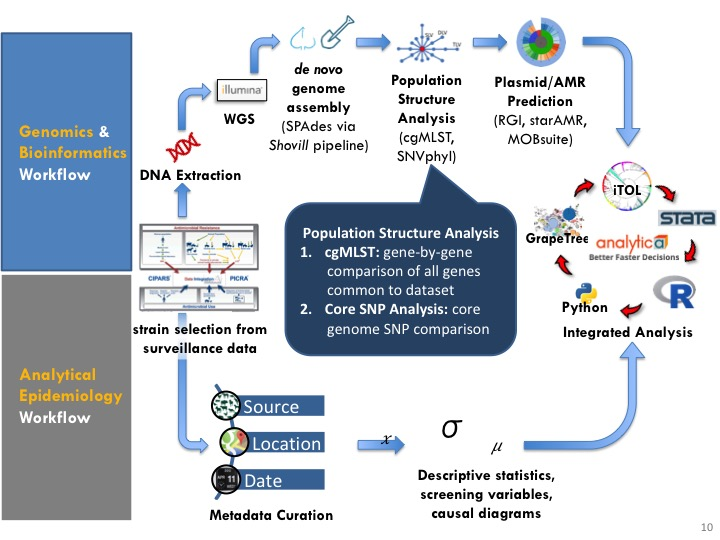
\includegraphics[width=\textwidth]{figures/analysisworkflow.jpg}

        \caption{Flowchart describing the workflow of data analyses and bioinformatics pipelines}

        \label{fig:Analysis Workflow}

\end{figure}

\section{Anticipated Significance}


At the most basic level, this research aims to further the understanding of the potential role that raccoons may play in the epidemiology of \textit{Campylobacter jejuni}. Raccoons may be relevant in the spread of \textit{Campylobacter} amongst farms through their access to livestock and agricultural plants.

At the more fundamental level, however, the approaches developed to analyze the whole genome sequencing data obtained from the \textit{Campylobacter}-positive raccoon population will be applicable to analyzing whole genome sequence data of other \textit{Campylobacter} populations and provide guidance on analytical approaches for \textit{Campylobacter} whole genome sequence data.
%aims to be applicable to other \textit{Campylobacter} populations and to act as a guide to analyzing whole genome sequence data. 
The methods used for analyzing the genomic diversity and the strain dynamics %carriage?
within this raccoon population will prove useful for the analysis of human sporadic cases and outbreaks. 



%- *Campylobacter* in raccoons significance -> draw a line between previous mention of raccoon vector 


%- develop raccoon dataset epidemiological model of *Campylobacter* circulating in a population 

 % - surveillance of *Campylobacter* in humans is limited; need to develop approaches applicable to human surveillance 
  
  %    - incomplete data to answer questions on genomic diversity and epidemiology
 
  %- guideline for analyzing WGS human data 
      
   %   - use methods for genomic diversity and carriage analyses as guidelines for examining *Campylobacter* in humans 



\newpage
\small

%\bibliography{References}
\printbibliography


\end{document}